\documentclass[11pt,a4paper]{article}

\usepackage[T1]{fontenc}
\usepackage[utf8]{inputenc}
% lmodern unavailable in this TeX tree; arXiv has it. Uncomment before submission:
% \usepackage{lmodern}
\usepackage[margin=1in]{geometry}
\usepackage{amsmath,amssymb}
\usepackage{booktabs}
\usepackage{array}
\usepackage{longtable}
\usepackage{url}
\usepackage[hidelinks]{hyperref}
\usepackage{xcolor}
\usepackage{enumitem}
\usepackage{caption}
\usepackage{pgfplots}
\pgfplotsset{compat=1.17}
\usepackage[expansion=false]{microtype} % expansion needs scalable fonts; arXiv has lmodern, drop the option there

\captionsetup{font=small,labelfont=bf}
\setlist{nosep,leftmargin=*}
\newcommand{\code}[1]{\texttt{\small #1}}

\title{\bfseries What Physical Layout Determines in a Document Store:\\
Capability and Index Currency, Not Latency\\
\large\normalfont Evidence from seven measurement campaigns,
with the artefact and its own refutations}

\author{%
  David Leconte\\
  \small IBM France\\
  \small \texttt{github.com/davidleconte/shredding-cost-hcd-mongodb}%
}

\date{19 September 2026}

\begin{document}
\maketitle

\begin{abstract}
\noindent
A document database may store each record whole or decompose it into typed columns with
automatically maintained secondary indexes. We ask what that choice determines. Across seven
measurement campaigns against one build of each of two systems, we find that physical layout
predicts two things reliably and a third unreliably. It predicts \emph{which operations exist}:
the decomposing interface we examined exposes no server-side aggregation, refuses exact counts
above a documented threshold, and returns an estimate in error by roughly fourteen percent in
steady state --- all structural facts, independent of hardware and load. It predicts \emph{when a
search index is current}: searching immediately after a write, the comparator
\emph{missed} the document in $30/30$ trials and the decomposing engine in $0/30$ --- a difference
exactly tested at $p \approx 8.5\times10^{-18}$; the asymmetry vanishes entirely once the delay exceeds the
comparator's refresh interval. It does \emph{not} reliably predict latency, and we establish this
negatively: of 93 pairwise comparisons re-analysed by separation of support, 56 separate,
34 overlap and 3 cannot be decided at all, and among the overlapping are two of the three margins
favouring the decomposing engine. We further show that the study's
headline ratios --- quotients of fitted slopes --- have no finite upper bound on one of the two
passes collected, the denominator being indistinguishable from zero. We report a methodological
consequence: on the index-currency axis, a comparison of \emph{latencies} fails to separate while a
comparison of \emph{proportions} on the same trials separates completely, because the two latencies
are not values of one quantity. The measurement envelope is narrow --- one shared host, a single
sequential closed-loop client, 200{,}000 to 1{,}000{,}000 documents, one datacentre --- and is the
envelope in which the decomposing engine is weakest. All raw records, probe sources, adversarial
audits and integrity checks are published, and for each claim we pre-declare the measurement that
would overturn it.
\end{abstract}

\vspace{0.5em}
\noindent\textbf{Keywords:} document stores; secondary indexing; index currency; read-your-writes;
LSM storage; measurement methodology; limits of latency measurement.

\vspace{0.5em}
\noindent\textbf{Conflict of interest.} The author is employed by a company that resells both
systems examined and works on one of them. The system he works on loses five of the eight axes
reported. Every figure is published with the reserve that bounds it, the raw records are unedited,
and the adversarial audits written against this work are published alongside it.

\section{Introduction}

A document database must decide where a record lives on disk. One family stores each document
approximately as presented, in a binary encoding, and indexes only what the operator declares.
Another decomposes the document at write time into generic typed columns, and maintains secondary
indexes over them without instruction --- the wide-column lineage of Bigtable~\cite{chang2008bigtable}
and Cassandra~\cite{lakshman2010cassandra}, over an LSM store~\cite{oneil1996lsm,luo2019lsmsurvey}. The second arrangement is not exotic: it is how a document
API layered over a wide-column engine reconciles a schemaless interface with a schema-bearing store.

The trade is usually described qualitatively. Decomposition makes every field queryable without
declaration and makes the record searchable at acknowledgement; it charges index maintenance to
every write. Whole-record storage charges nothing it was not asked to and keeps search indexing off
the transaction path; a search issued immediately after a write may not find it.

This note asks what that choice \emph{determines}, and separates three answers.

\begin{description}[style=nextline]
\item[It determines capability.] Whether an operation exists at all --- aggregation, exact
counting, grouping off the partition key --- is settled by the interface and the storage model, not
by hardware. These results need no percentile and survive every objection about sample size.

\item[It determines index currency.] Whether a search finds what was just written is a property of
where index maintenance sits relative to the commit. We measure it as a \emph{failure rate} against
delay, which is exactly testable, rather than as a latency, which on these data is not.

\item[It does not determine latency, on evidence we can offer.] We report this as a negative
result with its mechanism: our own apparatus cannot establish direction on 34 of 93 comparisons,
our headline slope ratios are unbounded on one of two passes, and the coefficient we published
first collapses by a factor of five between cache regimes.
\end{description}

\paragraph{Contributions.}
\begin{enumerate}
\item Five structural properties of a decomposing document API, measured or located in vendor
documentation, three of them not stated in that documentation: a consensus round on every mutation;
an 8{,}000-byte ceiling on indexed strings; nine automatic indexes per collection against a
hundred-per-node guardrail; no server-side aggregation; and an estimator wrong by $\approx 14\%$
after both flush and major compaction (\S\ref{sec:capability}).
\item An exactly tested measurement of index currency as a miss-rate curve, and the observation
that the same phenomenon does not separate as a latency comparison, with the reason
(\S\ref{sec:currency}, \S\ref{sec:forms}).
\item \textbf{A result about measurement rather than about engines}, which we believe transfers
furthest: on one phenomenon, measured in one set of trials, a comparison of \emph{latencies} fails to
separate while a comparison of \emph{proportions} separates completely --- because the two latencies
are not values of one quantity, one being a transport floor and the other an indexing schedule. The
overlap is therefore not noise to be beaten with a larger sample; the comparison was ill-posed
(\S\ref{sec:forms}).

\item A distribution-free re-analysis of 93 comparisons by separation of support, applicable to any
study whose per-observation series were discarded, together with the finding that this apparatus
cannot reach the study's own headline quantities (\S\ref{sec:inference}).
\item A published artefact containing the raw records, the probe sources, nine automated integrity
checks, and the adversarial audits that reversed several of our own conclusions
(\S\ref{sec:artefact}).
\end{enumerate}

\paragraph{What this note is not.} It is not a benchmark. Load was driven closed-loop by a single
client throughout; no concurrency was measured; the systems ran on one shared host under
uncontrolled background load. A reader seeking throughput or tail behaviour under contention will
find nothing usable here, and \S\ref{sec:threats} says so in the terms a reviewer would use.

\section{Setting and method}
\label{sec:method}

\paragraph{Systems.} The decomposing side is \textbf{IBM DataStax Hyper-Converged Database 2.0.6}
(release \code{5.0.7.0-ea50e91ba01f}), a Cassandra-derived wide-column engine, addressed through its
\textbf{Data API v1.0.33}. The whole-record side is \textbf{MongoDB 8.0.32}, a three-member replica
set. For the index-currency axis only, MongoDB ran as \code{mongodb-atlas-local} 8.3.11 carrying
\code{mongot} 1.75.1 in the \code{localDev} edition, which its vendor designates for evaluation
rather than production --- a substitution we flag wherever a result depends on it.

We name the products because the capability findings of \S\ref{sec:capability} are checkable only
against named documentation, and because the artefact names them throughout. Elsewhere in this note
we write \emph{decomposing engine} and \emph{comparator}, not from discretion but because the thesis
concerns a \emph{physical arrangement} rather than two brands: a reader operating some other
decomposing document interface should be able to ask which of these results transfer.

\paragraph{Corpus and workload.} The mutation series uses synthetic documents of a single shape:
an identifier, one short mutable status field, and sixteen ballast strings of equal length, the
length varying across the series at 512, 1{,}024, 2{,}048, 4{,}096 and 8{,}000 bytes --- so documents
of roughly 8, 16, 32, 64 and 128\,KB, with field \emph{count} held constant and indexed \emph{volume}
varying. The mutation under test is always the same: one \code{\$set} on the status field, which
touches none of the ballast. The 8{,}000-byte ceiling is not a design choice but the largest indexed
string the decomposing interface accepts, which is why the series stops there and why wider
documents are reached by adding bytes per field rather than fields.

A second corpus, used for the capability and aggregation axes, holds 200{,}000 documents carrying a
category drawn from ten values and a deterministic numeric amount, so that every aggregate has a
ground truth computed independently in the probe and every arm is verified exact against it before
its timing is reported. Holding field count fixed while varying bytes is what lets
\S\ref{sec:inference} attribute the mutation cost to indexed volume rather than to field count --- a
separate series, varying the count at constant volume, returned \emph{inconclusive} against its
pre-registered threshold and is reported as such in the artefact.

\paragraph{Host and regime.} One shared virtual machine, 80 vCPU, 220\,GiB RAM, at load average
14--16 throughout; storage class not establishable. Six of seven campaigns ran cache-resident. Two
campaigns reached disk: one placed the dataset beyond memory, and one re-measured the aggregation
axis after an explicit flush and a major compaction.

\paragraph{Durability mapping.} Majority write concern with journalling on the comparator against
quorum-level writes with a periodic commit-log sync on the decomposing engine. This mapping
\emph{favours} the decomposing engine, which acknowledges before its sync while the comparator
waits for its journal. We adopted it deliberately: the decomposing engine lost the mutation axis
anyway, and a reader may discount the margin accordingly.

\paragraph{Statistics.} Percentiles only; no means for latency. Thirty observations per point, two
passes at most. Of the thirty-nine raw records the probes wrote, twenty-five carry latency
distributions, and \textbf{twenty-three of those twenty-five discarded their per-observation series
at write time}, keeping only summaries. No confidence interval is recoverable from them by anyone,
including the author. The two records that retain their observations belong to the final campaign,
and they publish bootstrap intervals over the retained series.

What survives universally is one distribution-free question: are the two arms' observed ranges
disjoint? Where they are, every observation of one arm beat every observation of the other, and the
direction follows without any distributional assumption; the exact one-sided permutation
probability of that outcome is $1 / \binom{n_A + n_B}{n_A}$. We apply it to all 93 comparisons and
report the answer for every axis.

\section{Layout determines capability}
\label{sec:capability}

Five properties of the decomposing interface bear on design and are independent of hardware, load
and cache regime.

\begin{enumerate}
\item \textbf{A consensus round on every mutation.} Tracing shows each single-field update compiled
into a read followed by a conditional rewrite of the whole document and its derived columns, the
conditional executing at serial consistency. This is not optional and not configurable through the
interface. \emph{Reserve:} every probe in this work emits conditional updates, including the direct
arm intended to remove the interface, so the cost of consensus is nowhere isolated.

\item \textbf{An 8{,}000-byte ceiling on any indexed string.} Exceeding it is refused at write time,
which forced chunking in our own document generator and makes selective indexing compulsory for
long text.

\item \textbf{Nine automatic indexes per collection, against a hundred-per-node guardrail.} About
eleven collections per node before creation is refused --- a capacity limit imposed by an indexing
convenience rather than by data volume.

\item \textbf{No server-side aggregation.} The command allow-list on this build holds nineteen
commands; \code{aggregate}, \code{\$group} and \code{distinct} answer \code{COMMAND\_UNKNOWN}.
Summing a field by category therefore has exactly one route through the interface: transfer the
corpus to the client. \emph{Reserve:} an allow-list is a product decision and can change between
builds; what resists is the mechanism, not the list.

\item \textbf{Exact counting refused, and the estimator wrong in steady state.} The vendor documents
that exact counts beyond a threshold are unsupported and recommends the estimate. On this build the
threshold is a thousand. The recommended estimate returned \textbf{0} for a collection holding
200{,}000 documents before the first flush; re-measured after a flush it returned 171{,}267, and
after a major compaction 172{,}132 --- errors of $14.4\%$ and $13.9\%$, not converging. The
comparator's estimator returned 200{,}000 exactly on the same corpus.
\end{enumerate}

\paragraph{A limit of expressibility, measured.} The native query language offers grouping, but only
on primary-key columns. Against a table whose primary key does not carry the group column,
\code{GROUP BY} is refused outright (\code{InvalidRequest code=2200}), with or without a filtering
hint. The escape from the missing aggregation pipeline therefore presupposes a table partitioned by
the group key in advance. \emph{Reserve, pre-registered and triggered:} the per-partition sweep,
which is the faster of the two native routes, does execute against an unpartitioned table once a
filtering hint is added. What is categorically inexpressible without pre-partitioning is the
grouping form alone.

\paragraph{Is this a fair axis?} The engine's own modelling doctrine instructs the reader not to
aggregate at query time but to store pre-computed answers, roughly a table per query. The
architecturally correct response to ``sum this field by category'' is thus \emph{neither} route we
measured. What keeps the measurement meaningful is that the subject is the \emph{interface}, whose
proposition is document ergonomics in the manner of the comparator; a team adopting it on that basis
will expect \code{aggregate} and will meet its absence at a \code{COMMAND\_UNKNOWN}. The comparison
is fair at the API surface and unfair at the storage engine, and both halves must travel together.

\paragraph{Magnitude, with its condition.} Where the operation exists on both sides, the cost of the
missing pipeline is large and \emph{depends on the query}. Against a client-side scan of 200{,}000
documents (median 132{,}985\,ms, $n=15$), the comparator's server-side grouping took 227.5\,ms at
ten groups, 878.2\,ms at a hundred thousand groups, and 218.4\,ms filtered-then-grouped --- ratios
of $584\times$, $151\times$ and $609\times$ respectively, on disjoint bootstrap intervals. The
comparator's cost follows group cardinality; the interface's does not, being dominated by transport.
\textbf{The ratio falls by a factor of 3.9 across that range}, so no single multiplier should be
quoted.

\section{Layout determines index currency}
\label{sec:currency}

Write a document, then search for it after a delay $\tau$. Does the search find it?

\begin{table}[htbp]
\centering
\small
\caption{Miss rate at nine delays, thirty trials each, both systems on one host. A miss is a search
that does not return a document already acknowledged as written. Figure~\ref{fig:miss} plots these
same counts.}
\label{tab:miss}
\begin{tabular}{lrrrrrrrrr}
\toprule
$\tau$ (ms) & 0 & 100 & 250 & 500 & 750 & 1000 & 1500 & 2000 & 3000 \\
\midrule
Decomposing engine & 0/30 & 0/30 & 0/30 & 0/30 & 0/30 & 0/30 & 0/30 & 0/30 & 0/30 \\
Comparator         & 30/30 & 28/30 & 25/30 & 15/30 & 10/30 & 0/30 & 0/30 & 0/30 & 0/30 \\
\bottomrule
\end{tabular}
\end{table}

\begin{figure}[htbp]
\centering
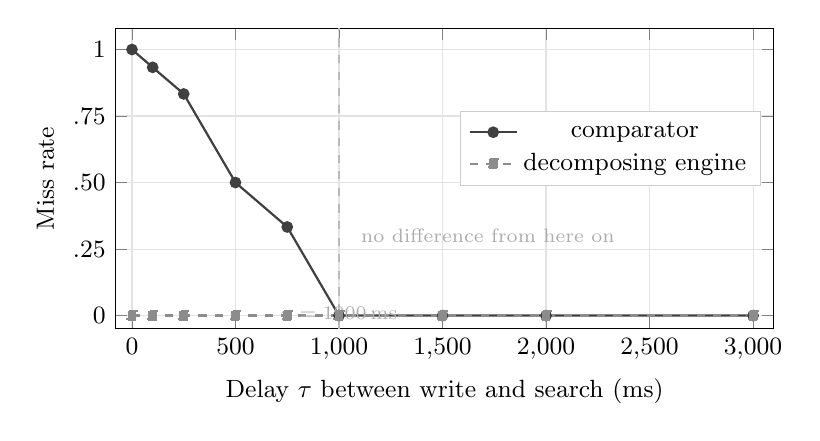
\begin{tikzpicture}
\begin{axis}[
  width=0.82\textwidth, height=5.4cm,
  xlabel={Delay $\tau$ between write and search (ms)},
  ylabel={Miss rate},
  xmin=-80, xmax=3100, ymin=-0.05, ymax=1.08,
  ytick={0,0.25,0.5,0.75,1}, yticklabels={0,.25,.50,.75,1},
  xtick={0,500,1000,1500,2000,2500,3000},
  grid=major, grid style={gray!22},
  legend style={at={(0.98,0.60)},anchor=east,draw=gray!40,font=\small,fill=white},
  tick label style={font=\small}, label style={font=\small},
  every axis plot/.append style={thick},
]
\addplot[mark=*,mark size=1.7pt,color=black!75] coordinates {
 (0,1.000) (100,0.933) (250,0.833) (500,0.500) (750,0.333)
 (1000,0) (1500,0) (2000,0) (3000,0)};
\addlegendentry{comparator}
\addplot[mark=square*,mark size=1.6pt,color=black!45,dashed] coordinates {
 (0,0) (100,0) (250,0) (500,0) (750,0) (1000,0) (1500,0) (2000,0) (3000,0)};
\addlegendentry{decomposing engine}
\draw[gray!55,dashed] (axis cs:1000,-0.05) -- (axis cs:1000,1.08);
\node[anchor=west,font=\scriptsize,gray!65] at (axis cs:1060,0.30)
  {no difference from here on};
\node[anchor=south,font=\scriptsize,gray!65] at (axis cs:1000,-0.05)
  {$\tau=1000$\,ms};
\end{axis}
\end{tikzpicture}
\caption{The data of Table~\ref{tab:miss}, thirty trials per point. The transition tracks the
comparator's refresh interval --- measured at mean 646.3\,ms over sixty trials (min 89.1,
max 1170.2) --- and not its identity: a deployment with a different interval moves the curve. The
curve's existence is the structural fact; its position is a setting. At $\tau=0$ the separation is
complete and exactly tested; from $\tau=1000$\,ms the two arms are indistinguishable.}
\label{fig:miss}
\end{figure}

At $\tau = 0$ the separation is total: Fisher's exact test gives a one-sided
$p = 8.456\times10^{-18}$, which is exactly $1/\binom{60}{30}$ --- the probability floor set by the
design rather than by the effect, the effect being complete. From $\tau = 1000$\,ms onward there is
no difference at all.

The transition tracks the comparator's \emph{refresh interval}, not its identity. Measured without
phase-locking onto the refresh cycle, that interval had mean 646.3\,ms over sixty trials
(min 89.1, median 664.3, max 1170.2). A deployment with a different interval would move the curve;
the curve's existence is the structural fact, its position is a setting.

\paragraph{The decision rule this yields.} Two numbers decide this axis, and only one concerns a
database: the refresh interval of the deployment, and the delay the application leaves between
writing and searching. Where the second is shorter than the first, the decomposing engine returns
the document and the comparator does not. Where it is longer, the advantage is worth nothing.

\paragraph{Reserves.} The comparator's search process ran in an evaluation edition in a single-node
container; a production topology places search on dedicated nodes and may refresh differently, in
either direction. The two search paths are not the same object --- one lexical, one vector --- and
we compare \emph{currency}, not retrieval quality. The decomposing engine's ``synchronous'' is
bounded below by an HTTP floor of $\approx$45\,ms, so we can establish that its window is smaller
than one measurement floor, not that it is zero.

\section{Layout does not reliably determine latency}
\label{sec:inference}

We state this negatively, with three pieces of evidence, two of them against our own headline
numbers.

\paragraph{(a) A third of the comparisons do not separate, and three cannot be judged.} Of 93
pairwise comparisons re-analysed by separation of support, 56 are disjoint, \textbf{34 overlap}, and
\textbf{3 are undecidable}: their records kept a median and nothing else --- no count, no minimum,
no maximum --- so neither separation nor any interval can be computed from them. Two of those three
are the disk-regime comparisons, which is to say that the regime evidence on which
\S\ref{sec:inference}(c) rests is the evidence least able to defend itself. We report the coefficient
collapse as a fact about two medians and nothing more. Among the overlapping are two of
the three margins that favour the decomposing engine. In particular, on filtering by a field nobody
declared --- the axis automatic indexing exists to serve --- the comparator's fastest of fifty
observations (13.3\,ms) beats the decomposing engine's median (17.4\,ms), and the ratio interval
runs $[0.46, 65.8]$, containing one. What these data establish there is \emph{predictability}
($\approx$17\,ms whatever the document, against 13--863\,ms) and not speed.

\paragraph{(b) The headline ratios are unbounded on the pass that was not used.} The most quotable
numbers in this work are quotients of fitted slopes. The distribution-free apparatus above compares
samples and fits nothing; it therefore reaches none of them. Fitting both passes and propagating
standard errors:

\begin{table}[htbp]
\centering
\small
\caption{Denominator slopes (ms per indexed KiB) and the ratio to the decomposing engine, by pass.
The harness fitted pass one only; nothing in earlier revisions of this work said so.}
\label{tab:slopes}
\begin{tabular}{lcc}
\toprule
 & Pass one & Pass two \\
\midrule
Comparator, wildcard index        & $0.0176 \pm 0.0038$ & $\mathbf{0.0063 \pm 0.0026}$ \\
Comparator, nothing declared      & $0.0098 \pm 0.0030$ & $\mathbf{0.0085 \pm 0.0058}$ \\
Ratio, wildcard arm               & $44\times$          & $\mathbf{116\times}$ \\
Fieller interval on that ratio    & $[26, 142]$         & \textbf{unbounded} \\
\bottomrule
\end{tabular}
\end{table}

On pass two the denominator's interval reaches zero, so by Fieller's theorem~\cite{fieller1954ratio}
the ratio has no finite upper bound; the
point estimate moves by a factor of 2.6 between two passes of one probe on one machine.
\textbf{No value of this ratio is publishable.} What is defensible is a range of latencies:
roughly threefold at 8\,KB widening to thirteenfold at 128\,KB, on supports disjoint in 19 of 20
size-and-pass cells.

\paragraph{(c) The regime moves the coefficient by a factor of five.} The per-byte mutation
coefficient we first published is $\times 7.50$ with the dataset memtable-resident, $\times 5.94$
with it on disk, and $\times 1.52$ once a flush before each update forces the read half of the
read-modify-write cycle onto the storage layer. \textbf{A single ``cost per KiB'' for an LSM-backed
document store is therefore not a well-formed number.} The mechanism transfers; the rate does not.

\section{One phenomenon, two forms of the question, two verdicts}
\label{sec:forms}

Section~\ref{sec:currency} reports index currency as a proportion. As a comparison of
\emph{latencies} on the same trials, the two arms' observed ranges overlap --- the decomposing
engine's maximum (573.6\,ms) exceeds the comparator's minimum (89.1\,ms) --- and the ratio interval
$[0.16, 36.7]$ contains one. Same runs, same corpus, opposite verdicts.

The proportion binds, and the reason is not that users care more about failures than about waiting.
It is that \textbf{the two latencies are not values of one quantity}. The $\approx$45\,ms on one
side is a measurement floor, the round trip carrying the question; the $\approx$646\,ms on the other
is a refresh interval, a property of an indexing schedule. Subtracting one from the other subtracts
a transport from a timetable. The overlap that defeats the latency comparison is therefore not noise
to be beaten with more observations: the comparison was ill-posed, and no sample size repairs it.
The proportion asks one well-posed question of both --- \emph{at this instant, is the document
there?} --- and both answer in the same units.

We state the generalisation cautiously, since it rests on one instance: where a comparison refuses
to separate, it may be worth asking whether the two arms measure the same quantity before concluding
that the effect is small.

\section{Summary of axes}
\label{sec:summary}

\begin{table}[htbp]
\centering
\small
\caption{Eight axes on which the two systems were set against each other, with the inference status
of each. ``Certain'' means the two arms' observed ranges are disjoint. Rows come from four
deployment configurations and are not commensurable with one another; the count is not a score.}
\label{tab:axes}
\begin{tabular}{p{4.6cm}p{2.5cm}p{7.2cm}}
\toprule
\textbf{Axis} & \textbf{Favours} & \textbf{Status and reserve} \\
\midrule
Mutating one field & comparator & Certain (disjoint in 19/20 cells). Memtable-regime; slope ratios
unpublishable (\S\ref{sec:inference}) \\
Fetching by identifier & comparator & Certain. Much of the gap is the interface's HTTP hop, not
isolated on the read path \\
Filtering, declared index & comparator & Certain \\
Aggregating by group & comparator & \textbf{Capability}, not a race: no server-side pipeline. Ratio
depends on group cardinality ($584\times$ to $151\times$) \\
Counting exactly & comparator & \textbf{Structural}: the operation is refused; the estimator is
wrong by $\approx 14\%$ in steady state \\
Freshness, ordinary index & neither & Both current at first query, 40/40 each \\
Filtering, undeclared field & \textbf{not established} & Supports overlap, interval $[0.46, 65.8]$.
What is established is predictability \\
Freshness, search index & decomposing engine & Certain \emph{as a proportion}
($p \approx 8.5\times10^{-18}$); \textbf{not established as a latency}. Total inside the refresh
window, void outside \\
\bottomrule
\end{tabular}
\end{table}

\section{Threats to validity}
\label{sec:threats}

\paragraph{Construct.} ``Cost'' is latency throughout, never bytes written. A layout property
estimated through a latency proxy inherits the cache state of the run, which is why the flagship
coefficient spans a factor of five across three regimes. The capability results
(\S\ref{sec:capability}) are untouched by this, being non-latency measurements.

\paragraph{Statistical conclusion.} Per-observation series were discarded by 23 of the 25
latency-bearing records; the remaining two are the final campaign's. No interval, no test and no
re-percentiling is possible for the other twenty-three, for any reader, permanently. What the surviving minima and maxima decide is overlap, and 34 of 93 comparisons
overlap.

\paragraph{Internal.} Instruments were written by the measurer. The comparisons that fail separation
of support and the measurements carrying no pre-registered decision rule are largely the same rows,
and they are disproportionately the rows favourable to the author's employer's product. We report
the overlap rather than the medians for those rows.

\paragraph{External.} One host, one build of each system, one datacentre, 200{,}000 to 1{,}000{,}000
documents, a single sequential closed-loop client. \textbf{This envelope is the one in which the
decomposing engine is weakest and the comparator strongest:} nothing that makes the architectural
case for a distributed engine --- partitioning at scale, sustained concurrent writes, multi-site
replication --- was exercised once. Three regimes could change the picture and none was measured:
beyond one node's memory; beyond the write load one deployment absorbs; and across datacentres,
where two effects (a costlier consensus round, and a single-replica vector read) would both tell
\emph{against} the decomposing engine.

\paragraph{Closed loop.} Load was driven closed-loop throughout, which is the first pitfall the
benchmarking literature names~\cite{schroeder2006openclosed,raasveldt2018fair}: the sampling rate is a
decreasing function of latency, so slow periods contribute proportionally fewer observations. Published tail percentiles are tails of a service-time
distribution at negligible utilisation, not of a response-time distribution under load, and carry none
of the meaning tail latency has in a served system~\cite{dean2013tail}.

\paragraph{Editions.} The comparator's search process was measured in an evaluation edition. Two
documentation pages cited for the decomposing engine belong to an earlier documentation line than
the build measured; both citations are flagged in the artefact.

\section{What would overturn each claim}
\label{sec:falsify}

A study that declares its limits should also declare what would settle them. Each row below names
the measurement that would refute the corresponding claim, so that a reader who disagrees knows what
to run rather than what to argue. None of these was performed here.

\begin{table}[htbp]
\centering
\small
\caption{Pre-declared refutation conditions. Rows are ordered by how cheap the refuting measurement
is to perform.}
\label{tab:falsify}
\begin{tabular}{p{4.3cm}p{9.8cm}}
\toprule
\textbf{Claim} & \textbf{What would overturn it} \\
\midrule
No server-side aggregation (\S\ref{sec:capability}) &
A build of the same interface answering \code{aggregate} or \code{\$group} without
\code{COMMAND\_UNKNOWN}. An allow-list is a product decision; one release closes this. \\
Exact counting refused above a threshold &
A configuration parameter raising or removing the threshold. We searched for one and found none;
finding one refutes the claim as stated, not the behaviour we observed. \\
The estimator is wrong in steady state &
The same estimate converging on a larger corpus, or after more compaction passes than the one we
ran. Our two post-flush readings are a single trajectory, not a limit. \\
Index currency is total inside the window &
A production search topology --- dedicated nodes rather than a co-located evaluation edition ---
showing a miss at $\tau = 0$ on the decomposing side, or no miss on the comparator's. \\
The mutation gap widens with indexed volume &
A disk-bound series at the same sizes. Our disk campaign moved the coefficient by a factor of five
and did not repeat the full series; the direction is certain, the shape is not. \\
Layout does not determine latency &
Any of the above measured open-loop, on separate hosts, with per-observation series retained. That
is the measurement this study should have been, and its absence is why this claim is stated
negatively rather than positively. \\
\bottomrule
\end{tabular}
\end{table}

The last row is the important one. \textbf{This note does not claim that physical layout is
irrelevant to latency}; it claims that a study of this shape cannot establish the relation, and it
shows the arithmetic of why (\S\ref{sec:inference}). A better-instrumented study could establish
what this one could not, and the artefact exists so that it can be attempted against the same
probes.

\section{The artefact}
\label{sec:artefact}

The repository accompanying this note contains: 39 raw measurement records, unedited, including the
records of runs whose conclusions were later withdrawn; 19 probe sources; the derived inference file
containing all 93 comparisons with their supports and intervals; nine automated integrity checks run
in continuous integration (hashes, JSON validity, probe syntax, link resolution, figure
regeneration byte-for-byte, and cross-document agreement); and the adversarial audits, which are
written against the work and indexed so that a hostile reader can start there.

\paragraph{Entry point.} The cheapest verification requires no database at all: the derived
inference file states, for all 93 comparisons, the two arms' observed ranges and whether they are
disjoint, and a reader can recompute every verdict in this note from it and from the raw records
against which it is checked by continuous integration:

\begin{quote}\small\ttfamily
git clone --branch v1.0-arxiv \textit{<repository>} \&\& cd shredding-cost-hcd-mongodb\\
python3 .github/scripts/check\_evidence\_manifest.py\quad\textrm{\# every raw file matches its hash}\\
python3 .github/scripts/check\_inference.py\quad\textrm{\# every derived verdict re-derives}
\end{quote}

\noindent Reproducing the \emph{measurements} is a longer undertaking and needs both engines;
\code{REPRODUCING.md} carries the compose file and the prerequisites, and states plainly which parts
of the original environment were not recorded and therefore cannot be reconstructed --- the host port
mapping among them. Absolute latencies will not reproduce; the three refusals of
\S\ref{sec:capability} and the directions marked certain in Table~\ref{tab:axes} should.

Fifty-two numbered points record where measurement contradicted the text it was written to support.
They are kept as a list rather than a summary, because a summary would be a softening. Several
conclusions in earlier versions of this work were reversed by later campaigns, including two
reversals \emph{against} the author's initial reading; those reversals are in the text, not in
errata.

\section{Related work and position}

That secondary-index maintenance costs writes, and that a read-modify-write cycle costs more than a
blind write, are long established: the LSM literature analyses the write-amplification of index
maintenance directly~\cite{oneil1996lsm,luo2019lsmsurvey}, and the cost of distributed consensus on a
conditional write is the subject of~\cite{lamport1998parttime}. Neither is claimed here.

The methodological hazards we run into are equally well catalogued. Closed-loop generators are known
to misrepresent load~\cite{schroeder2006openclosed}, and the common pitfalls of cross-system database
measurement --- single hosts, unequal tuning, unreported regimes --- are enumerated
in~\cite{raasveldt2018fair}. We do not claim to have avoided them; we claim to have declared them and
to have reported what survives, following the threat taxonomy standard in empirical software
research~\cite{wohlin2012experimentation}.

\paragraph{The gap this note occupies.} Comparative measurement of these two engines is a populated
field, but every study we located compares Cassandra \emph{through CQL} to MongoDB through its own
driver: two query languages, two data models, two client stacks. We searched for published
measurement of a \emph{document API layered over a wide-column engine} --- the arrangement examined
here, in which the document model is a translation performed above the store rather than the store's
own model --- and found none, in the database venues or elsewhere. We state this as a search result
and not as a claim of priority: the absence may be ours. What follows from it is a caution about
transfer, which we make explicit in \S\ref{sec:threats}: results obtained through this interface are
properties of the \emph{translation} as much as of the engine beneath it, and our own direct-CQL arm
--- which removed the interface and left the consensus round standing --- shows how hard those two
are to separate.

What this note adds is narrower, and in three parts: a measured account of \emph{capability}
differences that a practitioner otherwise discovers in production; an exactly tested account of index
currency as a failure rate rather than a latency; and a worked demonstration that a study of this
shape cannot establish latency claims, with the arithmetic of why. The third is offered so that
comparisons of this kind can be read --- and written --- with the right expectations.

\bibliographystyle{plain}
\bibliography{refs}

\section*{Data availability}

All measurement records, probe sources, derived inference data and audit documents are available at
\url{https://github.com/davidleconte/shredding-cost-hcd-mongodb}, under CC-BY-4.0 for the documents
and data. \textbf{Every claim in this note refers to the state of that repository released as tag
\code{v1.0-arxiv}}; the repository's history has been rewritten during its development, so a bare
link to the default branch is not a stable reference and should not be treated as one. That release
is archived with a DOI, and \code{data/MANIFEST.sha256} carries one SHA-256 per raw record so that a
reader can verify the files individually against what this note reports. Absolute latencies will not reproduce on different hardware; the directions marked certain
in Table~\ref{tab:axes}, and the three refusals in \S\ref{sec:capability}, should.

\section*{Acknowledgements}

The adversarial audits that reversed several conclusions of this work were conducted with the
assistance of large language models, as was the drafting of the accompanying long-form articles.
Every measurement was executed by the probes published in the artefact; every reversal was checked
against the raw records by the author.

\end{document}
